\documentclass{beamer}

\usepackage[utf8]{inputenc}
\usepackage[english]{babel}

\usepackage{graphicx}
\usepackage{amsmath}
\usepackage{mathtools}
\usepackage{wrapfig}
\usepackage{amsfonts}
\usepackage{csquotes}
\usepackage{epigraph}
\usepackage{float}
\usepackage{lipsum}
\usepackage{blindtext}
\usepackage{multirow}
\usepackage[ruled,vlined]{algorithm2e}
\usepackage{bm}
\usepackage{xcolor}
\usepackage{upgreek}
\usepackage{calc}
\usepackage{lscape}
\usepackage[font={scriptsize}]{caption}
\usepackage{systeme}


% TYPESETTING SUGAR
\DeclareMathOperator*{\argmax}{argmax}
\DeclareMathOperator*{\argmin}{argmin}
\DeclareMathOperator*{\Find}{Find}
\DeclareMathOperator*{\find}{find}
\DeclareMathOperator*{\NNet}{NNet}
\DeclareMathOperator*{\EGR}{EGR}
\def\leq{\leqslant}
\def\geq{\geqslant}


\usetheme{Madrid}
\usecolortheme[rgb={0.0,0.4,0.5}]{structure}
%-----------------------------------------------%
%-----------------------------------------------%



%
% TITLE SLIDE
%

\makeatletter
\setbeamertemplate{footline}{%
  \leavevmode%
  \hbox{\begin{beamercolorbox}[wd=.4\paperwidth,ht=2.5ex,dp=1.125ex,leftskip=.20cm plus1fill,rightskip=.20cm]{author in head/foot}%
    \usebeamerfont{author in head/foot}\insertshortauthor
  \end{beamercolorbox}%
  \begin{beamercolorbox}[wd=.6\paperwidth,ht=2.5ex,dp=1.125ex,leftskip=.20cm,rightskip=.20cm plus1fil]{title in head/foot}%
    \usebeamerfont{title in head/foot}\insertshorttitle \hspace*{1.2ex}
    \insertframenumber{}/\inserttotalframenumber
  \end{beamercolorbox}}%
  \vskip0pt%
}
\makeatother

\title[\textit{Neural ODEs} for \textit{real-world}, irregularly-sampled, time series prediction]{\textit{Neural ODEs} \\ for \textit{real-world}, irregularly-sampled, time series prediction}

\author[E. Ballarin, M. N. Plasencia Palacios, A. Tasciotti]{Emanuele Ballarin \\ Milton Nicolás Plasencia Palacios \\ Arianna Tasciotti}
\institute[]{Department of Mathematics and Geosciences, University of Trieste}
\date[]{\textit{Statistical Machine Learning} course \\ Final Project $\sim$ June 2020}

\titlegraphic{
\includegraphics[width=1.25cm,height=1.3cm,keepaspectratio]{dssclogo.png}
	\hspace*{93.04mm}~% Horizontal space is tailored for 1.3cm square logos
	
\includegraphics[width=1.3cm,height=1.25cm,keepaspectratio]{logouniv.png}
}

%-----------------------------------------------%
%-----------------------------------------------%



%
% ADAPTIVE TABLE OF CONTENTS
%

\AtBeginSection[]
{
	\begin{frame}
		\frametitle{\textit{We are here...}}
		\tableofcontents[currentsection]
	\end{frame}
}

%-----------------------------------------------%
%-----------------------------------------------%



%
% DOCUMENT
%

\begin{document}

% Insert title slide
\frame{\titlepage}

%-----------------------------------------------%

%% TIME SERIES
%\section{Introduzione al paradigma del \textit{Deep Learning}}{
\section{\textit{Theory first!}}{

%% SLIDE 1.1:
\begin{frame}
\frametitle{Time Series}

A \textbf{time series} is a sequence of observations labeled in time order.  If the time-dependent variables are more than one we are talking about \textbf{multivariate time series}.\\~\

This type of data is highly exploited in economics, business and finance where it is important to predict future outcomes that depends on past observations.

\end{frame}
%---------------------------------------------%
%% SLIDE 1.2:
\begin{frame}
	\frametitle{RNN}
	%-----------------------------------------%
	To study a time series we can use a \textbf{Recurrent Neural Network} (RNN), which is a type of neural network in which the current hidden state is computed using the previous hidden state and the current input.

	 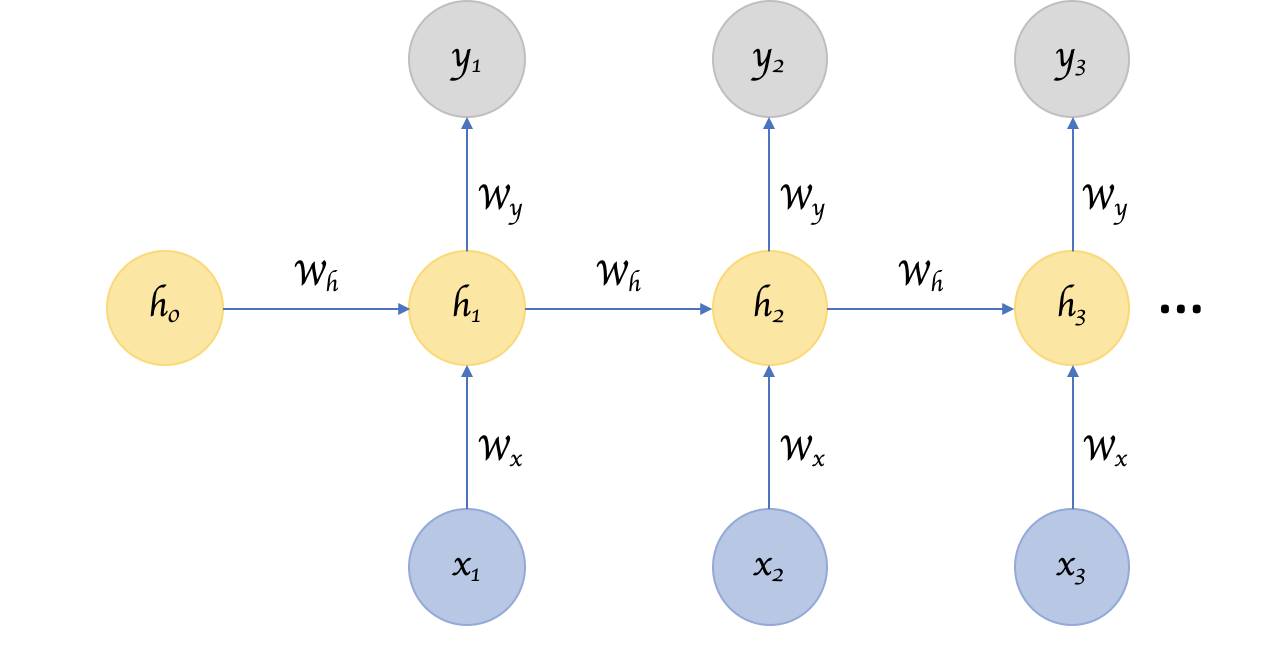
\includegraphics[scale = 0.25]{rnn1.png}
\end{frame}
%---------------------------------------------%
%%Slide 1.3.1
\begin{frame}
\frametitle{LSTM}

The \textbf{Long Short Term Memory Unit} is an improvement of the recurrent unit in which the information pass through a \textbf{don't forget gate} which decides to keep or throw away data. Input and output data are processed respectively by \textbf{input} and \textbf{output gate}.

\begin{center}
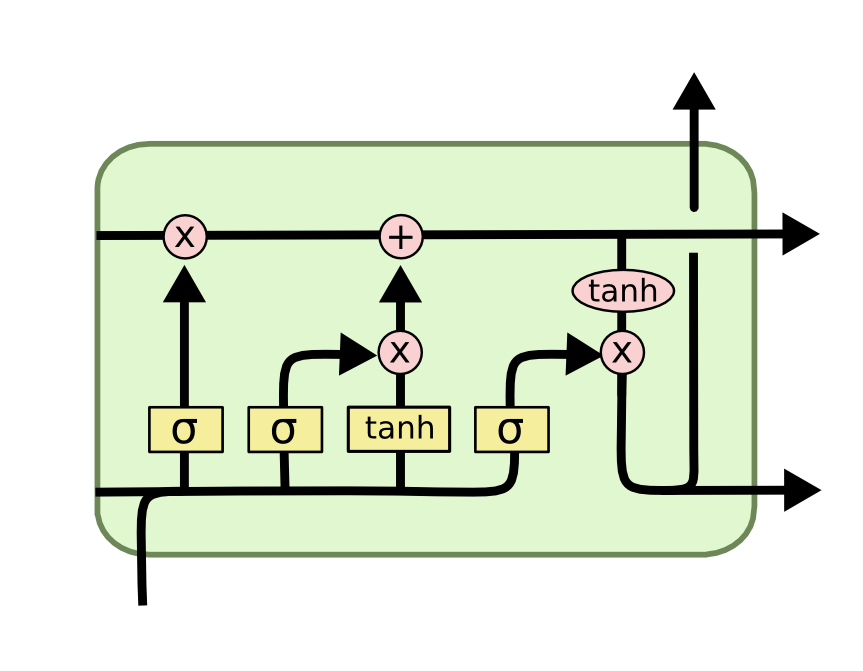
\includegraphics[scale = 0.5]{lstm.png}
\end{center}

\end{frame}
%---------------------------------------------%
%% SLIDE 1.3.2:
\begin{frame}
	\frametitle{GRU}
	\textbf{Gated Recurrent Unit} (GRU) is an improved version (in terms of efficiency) of the LSTM. GRU uses \textbf{update and reset gates} in order to modulate what information should be passed to the output.

	\begin{center}
	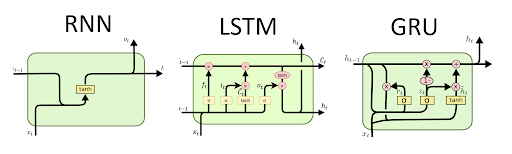
\includegraphics[scale = 0.6]{gru.png}
         \end{center}
\end{frame}
%---------------------------------------------%
%% SLIDE 1.4:
\begin{frame}
	\frametitle{ResNet}
	\textbf{Residual Neural Networks} (ResNet) use residual blocks and skip connections to solve vanishing gradient problem.

	\begin{center}
	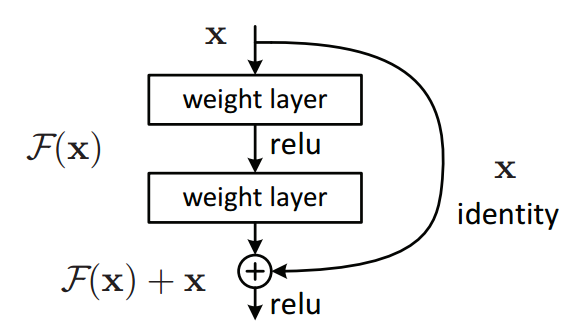
\includegraphics[scale = 0.4]{resnet.png}
         \end{center}

\end{frame}
%---------------------------------------------%
%% SLIDE 1.5:
\begin{frame}
	\frametitle{ODE}
	The ResNet model:

	\begin{equation}
	\textbf{h}_{l+1} =\textbf{h}_l + f(\textbf{h}_l, \theta_l)
	\end{equation}

	can be seen as  the Euler method for solving ordinary differential equations. We can exploit this new relation by adding more layers into the network and take smaller time steps.  In the limit we can describe our new neural network with the following model (\textbf{Neural ODE}):

	\begin{equation}
	\frac{d \textbf{h}(t)}{dt} = f(\textbf{h}(t), t, \theta)
	\end{equation}

	 with the function $f$ parameterized by a neural network, and solve it with a differentiable discretization method for ODEs.
\end{frame}
%---------------------------------------------%

%% SLIDE 1.6.1:
\begin{frame}
	\frametitle{RNN-ODE}
	\framesubtitle{Standard RNNs}
	\begin{figure}
	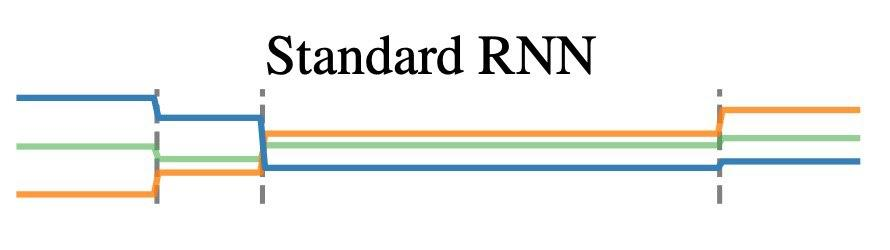
\includegraphics[height=0.24\linewidth]{standard_RNN.png}
	\caption*{'Latent ODEs for Irregularly-Sampled Time Series', Yulia Rubanova and Ricky T. Q. Chen and David Duvenaud, 2019.}
	\end{figure}
	\break
	\pause \begin{itemize}
	\item{Constant or undefined hidden states between observations}
	\end{itemize}
	\begin{itemize}
	\item{Hard to adapt for sparse irregular data...}
	\end{itemize}
\end{frame}
%---------------------------------------------%
%% SLIDE 1.6.2:
\begin{frame}
	\frametitle{RNN-ODE}
	\framesubtitle{RNNs for sparse data}
	\begin{itemize}
	\item{Include the time gap $\Delta_{t}=t_{i}-t_{i-1}$ between observations into RNN update function:}
	\end{itemize}
	$$h_{i} = RNNCell(h_{i-1}, \Delta_{t}, x_{i})$$
	\begin{itemize}
	\pause \item{Exponential decay of the hidden state:}
	\end{itemize}
	$$h_{i} = RNNCell(h_{i-1}, \exp{(-\tau \Delta_{t})}, x_{i})$$
	\begin{figure}
	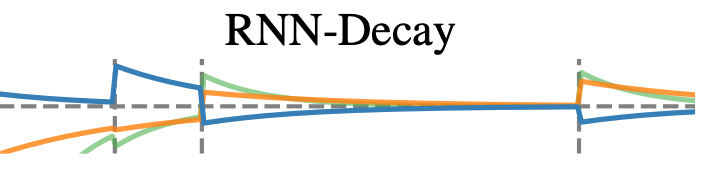
\includegraphics[height=0.18\linewidth]{RNN_decay.png}
	\caption*{'Latent ODEs for Irregularly-Sampled Time Series', Yulia Rubanova and Ricky T. Q. Chen and David Duvenaud, 2019.}
	\end{figure}
\end{frame}
%---------------------------------------------%
%% SLIDE 1.6.3:
\begin{frame}
	\frametitle{RNN-ODE}
	\framesubtitle{RNNs and Neural ODEs}
	Equivalence between exponential decay approach and solving an initial value problem involving an ODE:
	\[ \systeme[\frac{dh(t)}{dt} h(t_{0})]{\frac{dh(t)}{dt}=-\tau h, h(t_{0})=h_{0}} \]
	\hfill \break
	\pause ODE solution: $h(t)=h_{0}e^{-\tau \Delta_{t}}$
	\hfill \break
	\begin{itemize}
	\pause \item{hidden state $h(t)$ is an unknown function of time and is the solution of an ODE:}
	\end{itemize}
	$$\frac{dh(t)}{dt}=f_{\theta}(h(t),t)$$
	\begin{itemize}
	\pause \item{$h(t)$ can be evaluated at any time using a numerical ODE solver.}
	\end{itemize}
\end{frame}
%---------------------------------------------%
%% SLIDE 1.6.4:
\begin{frame}
	\frametitle{GRU-ODE architecture}
	The state between observations is the solution of an ODE:
	$$h_{i}^{'}=ODESolve(f_{\theta}, h_{i-1}, (t_{i-1},t_{i}))$$
	\hfill \break
	\pause For each observation, the hidden state is updated using a GRU update:
	$$h_{i}=GRUCell(h_{i}^{'},x_{i})$$
	\begin{figure}
	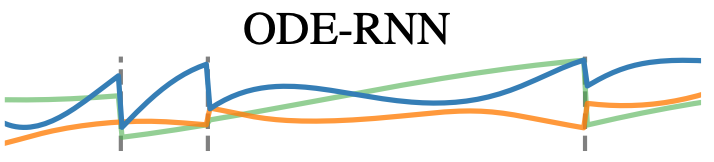
\includegraphics[height=0.16\linewidth]{ODE_RNN.png}
	\caption*{'Latent ODEs for Irregularly-Sampled Time Series', Yulia Rubanova and Ricky T. Q. Chen and David Duvenaud, 2019.}
	\end{figure}
\end{frame}
%-----------------------------------------------%
%% SLIDE 1.7:
\begin{frame}
	\frametitle{Latent ODE model}
	\begin{itemize}
	\item{Time series is represented by a latent trajectory;}
	\pause \item{Each trajectory is determined from a local initial state $z_{0}$ and a global set of latent dynamics shared across time series.}
	\end{itemize}
	\hfill \break
	\pause Two tasks:
	\begin{itemize}
	\item{extrapolation $\rightarrow$ forwards in time}
	\item{interpolation $\rightarrow$ backwards in time}
	\end{itemize}



%We investigate the ability of the latent ODE model to fit and extrapolate time series. The recognition network is an RNN with 25 hidden units. We use a 4-dimensional latent space. We parameterize the dynamics function f with a one-hidden-layer network with 20 hidden units. The decoder computing p(xti |zti ) is another neural network with one hidden layer with 20 hidden units. Our baseline was a recurrent neu- ral net with 25 hidden units trained to minimize negative Gaussian log-likelihood. We trained a second version of this RNN whose inputs were concatenated with the time difference to the next observation to aid RNN with irregular observa- tions.

\end{frame}
%---------------------------------------------%
%% SLIDE Intermezzo:
\begin{frame}
	\frametitle{Uncertainty quantifier}
	 \center $x_{in}$, $x_{out}$ observed, $z$ latent, $p(x_{in}, x_{out}, z)$ joint
	\pause \center $q(z_{0}|x_{in}, x_{out}) =  \mathcal{N}(\mu_{z_{0}},\sigma_{z_{0}})$
\end{frame}
}
%---------------------------------------------%
%% SLIDE 1.8:
\begin{frame}
	\frametitle{Uncertainty quantifier}
	\textbf{Feed-forward NN}
	\begin{itemize}
	 \item{Input: final hidden state of GRU-ODE}
	 \item{Output: $\mu_{z_{0}}$ and $\sigma_{z_{0}}$}
	\end{itemize}
	\hfill \break
	\pause \textbf{Sampler}
	\begin{itemize}
	 \item{Input: $\mu_{z_{0}}$, $\sigma_{z_{0}}$}
	 \item{Output: $\bar{z_{0}}$}
	\end{itemize}
\end{frame}
%---------------------------------------------%
%% SLIDE 1.9:
\begin{frame}
	\frametitle{Architectural overview}
	\center $h_{i}^{'}=ODESolve(f, h_{i-1}, (t_{i-1},t_{i}))$
	\center \pause $h_{i}=GRUCell(h_{i}^{'},x_{i})$
	\center \pause $\mu_{z_{0}}, \sigma_{z_{0}} =g(h_{i})$
	\center \pause $z_{0} \sim \mathcal{N}(\mu_{z_{0}},\sigma_{z_{0}})$
	\center \pause $\{z_{i}\}=ODESolve(z_{0}, f, (t_{0},...,t_{N}))$
	\center \pause $\widetilde{x_{i}}=OutputNN(z_{i})$

%Let x be a (set of) observed variable(s), z a (set of) latent variable(s) and let p(x, z) be the parametric model of their joint distribution, called the generative model defined over the variables. Given a dataset X = {x1 , ..., xN } we typically wish to perform maximum marginal likelihood learning of its parameters, i.e. to maximize XN i=1 but in general this marginal likelihood is intractable to compute or differentiate directly for flexible generative models, e.g. when components of the generative model are parameterized by neural networks. A solution is to introduce q(z|x), a parametric inference model defined over the latent variables, and optimize the variational lower bound on the marginal log-likelihood of each observation x:log p(x)  Eq(z|x) [log p(x, z)  log q(z|x)] = L(x; ✓)
\end{frame}
%---------------------------------------------%
\begin{frame}
	\frametitle{A \textit{bird's eye} architectural recap (1)}
	\framesubtitle{A \textit{lato sensu} encoder-decoder structure}
	\begin{block}{\center $h_{i}^{'}=ODESolve(f, h_{i-1}, (t_{i-1},t_{i}))$ \center $h_{i}=GRUCell(h_{i}^{'},x_{i})$}
		\centering
		\textit{Encoder}. Encodes an entire multidimensional, variable-length time series to fixed-low-dimensional latent representation, loop after loop. Outputs the present \textit{latent state}.
	\end{block}
	\center $\mu_{z_{0}}, \sigma_{z_{0}} =g(h_{i})$
	\center $z_{0} \sim \mathcal{N}(\mu_{z_{0}},\sigma_{z_{0}})$
	\center $\{z_{i}\}=ODESolve(z_{0}, f, (t_{0},...,t_{N}))$
	\center $\widetilde{x_{i}}=OutputNN(z_{i})$

\end{frame}
%---------------------------------------------%
\begin{frame}
	\frametitle{A \textit{bird's eye} architectural recap (2)}
	\framesubtitle{A \textit{lato sensu} encoder-decoder structure}
	\center $h_{i}^{'}=ODESolve(f, h_{i-1}, (t_{i-1},t_{i}))$
	\center $h_{i}=GRUCell(h_{i}^{'},x_{i})$

	\begin{block}{\center $\mu_{z_{0}}, \sigma_{z_{0}} = g(h_{i})$ \center $z_{0} \sim \mathcal{N}(\mu_{z_{0}},\sigma_{z_{0}})$}
		\centering
		\textit{Uncertainty estimator}. $\approx$ a VAE. Essentially \textit{BBVI} tricked into making uncertainty estimation (only). Outputs the present \textit{processed} latent state.
	\end{block}

	\center $\{z_{i}\}=ODESolve(z_{0}, f, (t_{0},...,t_{N}))$
	\center $\widetilde{x_{i}}=OutputNN(z_{i})$

\end{frame}
%---------------------------------------------%
\begin{frame}
	\frametitle{A \textit{bird's eye} architectural recap (3)}
	\framesubtitle{A \textit{lato sensu} encoder-decoder structure}
	\center $h_{i}^{'}=ODESolve(f, h_{i-1}, (t_{i-1},t_{i}))$
	\center $h_{i}=GRUCell(h_{i}^{'},x_{i})$
	\center $\mu_{z_{0}}, \sigma_{z_{0}} = g(h_{i})$
	\center $z_{0} \sim \mathcal{N}(\mu_{z_{0}},\sigma_{z_{0}})$

	\begin{block}{\center $\{z_{i}\}=ODESolve(z_{0}, f, (t_{0},...,t_{N}))$ \center $\widetilde{x_{i}}=OutputNN(z_{i})$}
	\centering
	\textit{Decoder}. Emits one entire predicted future-time-series, from present \textit{processed} latent state.
	\end{block}
\end{frame}
\section{\textit{Deep learning works great, except when it doesn't.}}{
%---------------------------------------------%
\begin{frame}
	\frametitle{The theory seems sound...}
	\framesubtitle{So sound it doesn't even work}
	\begin{figure}
		To make such architecture work in practice, we need to pull some (theoretically-grounded) tricks out of the $\widehat{trick}^*$!
	\end{figure}
\hfill\break
[* trick hat]
\end{frame}
%---------------------------------------------%
\begin{frame}
	\frametitle{\textit{Batch Normalisation} and \textit{Layer Normalisation}}
	\framesubtitle{A \textit{batch-wise} and a \textit{feature-wise} approach to training regularisation}

	Introduced to fight the problem of \textit{internal covariate shift}, they mainly act as \textit{noise-injection regularisers} \textit{(Leslie, 2019)}.
\hfill\break
	$$
	\hat{x}^{(j)}_i = \frac{x^{(j)}_i - \mu^{(j)}}{\sqrt{\sigma^{(j)^2} + \epsilon}}
	$$
	\begin{itemize}
		\item{\textit{BatchNorm (Ioffe, 2015)} acts dimension-wise over a minibatch, during training;}
		\item{\textit{LayerNorm (Ba, 2016)} acts dimension-wise and feature-wise, online, also during evaluation.}
	\end{itemize}
\end{frame}
%---------------------------------------------%
\begin{frame}
	\frametitle{Gradient Norm Clipping}
	\framesubtitle{Keeping seatbelts fastened}
	The recurrent nature of GRUs (and RNNs in general) may lead to exponentially-varying weights, and subsequently gradients. \\ $\rightarrow$ Training instability!
\hfill\break

\begin{itemize}
	\item{\textit{Vanishing gradients} $\rightarrow$ Gating (Schmidhuber, 1992; Cho, 2015), ReLU networks;}
	\item{\textit{Exploding gradients} $\rightarrow$ $ ||\nabla \boldsymbol{\theta}|| \coloneqq \text{min}(c, ||\nabla \boldsymbol{\theta}||)$ and rescale \textit{(Graves, 2013)}.}
\end{itemize}
\hfill\break
Also: no side effects if unneeded.

\end{frame}
%---------------------------------------------%
\begin{frame}
	\frametitle{AdamW Optimiser (1)}
	\framesubtitle{\textit{Ridge penalty} and \textit{weight decay} are not the same thing}
	All the \textit{Adam-family} optimisers:
	\begin{itemize}
		\item{Are Hessian-free;}
		\item{Use single-parameter-adaptive, upper-bound, SGD learning;}
		\item{Exploit $2^{nd}$-order gradient-momentum information.}
	\end{itemize}
\hfill\break
However, they regularise differently!
	\begin{itemize}
	\item{Adam: $\mathcal{L}_r = \mathcal{L} + \omega \frac{||\boldsymbol{\theta}||_2^2}{2}$ \textit{(Kingma, 2014)};}
	% w = w - lr * w.grad - lr * wd * w
	\item{AdamW: $\boldsymbol{\theta} \coloneqq \boldsymbol{\theta} - \boldsymbol{\rho}\cdot \nabla \boldsymbol{\theta} - \omega \boldsymbol{\rho}\cdot \boldsymbol{\theta}$ \textit{(Loshchilov, 2018)}.}
	\end{itemize}
\end{frame}
%---------------------------------------------%
\begin{frame}
	\frametitle{AdamW Optimiser (2)}
	\framesubtitle{A deeper dive into Adam \& friends}

	For each scalar weight $w$, at iteration $t$, in parallel:

	$$
	v_t = \beta_1 v_{t-1} - (1-\beta_1) \nabla w
	$$
	$$
	s_t = \beta_2 s_{t-1} - (1-\beta_2) (\nabla w)^2
	$$
	$$
	\rho = \text{min}\left({\text{lr}, \text{lr} \frac{v_t}{\sqrt{s_t + \epsilon}}}\right)
	$$
\hfill\break
	And then, the usual $\boldsymbol{\theta} \coloneqq \boldsymbol{\theta} - \boldsymbol{\rho}\cdot \nabla \boldsymbol{\theta}$.
\hfill\break
\hfill\break
Per-parameter estimation makes the two regularisations different.

\end{frame}

%-----------------------------------------------%
\begin{frame}
	\frametitle{$L_1$ loss}
	\framesubtitle{Uniformity is the key}
	An outright impopular choice for a loss function, however:
	\hfill\break
\begin{itemize}
	\item{The per-epoch loss average was $\approx 1$;}
	\item{$\mathcal{L}^2 < \mathcal{L}$ if $\mathcal{L} < 1$, whereas $\mathcal{L}^2 > \mathcal{L}$ if $\mathcal{L} > 1$, thus ruling out as potentially unstable and biased $L_2$ and \textit{Huber's smooth} losses;}
	\item{Also: more straightforward training monitoring (``$>2.5$'' heuristic)}
\end{itemize}
\end{frame}
}

\section{\textit{No data, no learning!}}{

%---------------------------------------------%
%% SLIDE 1.14:
\begin{frame}
	\frametitle{Dataset}
	The dataset contains informations about stock prices of many US companies in the period from 2 January 1962 to 27 March 2018.

	\begin{center}
	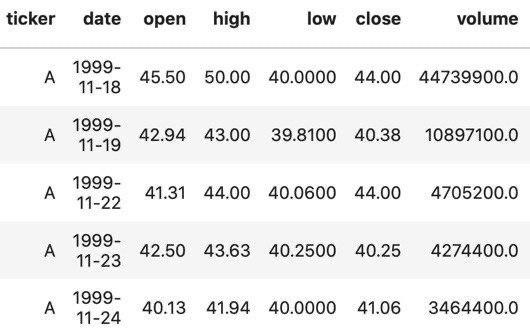
\includegraphics[scale = 0.40]{stock.jpg}
         \end{center}

\end{frame}
%---------------------------------------------%
\begin{frame}
	\frametitle{Windowing}
	\framesubtitle{Changing everything to make nothing change}

	Presenting data in overlapping-window form to RNNs is the first step to effectively \textit{teacher-force} them \textit{(Lamb, 2016; Hafner, 2018)}.

\begin{gather*}
a\ b\ c\ |\ d\ e\ f\ |\ g\ h\ i\ |\ \ \dots \\
b\ c\ d\ |\ e\ f\ g\ |\ h\ i\ j\ |\ \ \dots \\
c\ d\ e\ |\ f\ g\ h\ |\ i\ j\ k\ |\ \ \dots
\end{gather*}
(note: data ordered by column!)

\hfill\break

However, we often used very large windows to further improve learning on the most recent data.


\end{frame}
%---------------------------------------------%
\begin{frame}
	\frametitle{Data batching}
	\framesubtitle{You probably always made batches for RNNs wrong!}
	The second (and last) step is doing the batches in the right manner! \textit{(Lamb, 2016; Hafner, 2018)}.

\begin{gather*}
\alert{a\ b\ c}\ |\ \alert{d\ e\ f}\ |\ g\ h\ i\ |\ \ \dots \\
\alert{b\ c\ d}\ |\ e\ f\ g\ |\ h\ i\ j\ |\ \ \dots \\
\alert{c\ d\ e}\ |\ f\ g\ h\ |\ \alert{i\ j\ k}\ |\ \ \dots
\end{gather*}

\begin{itemize}
	\item{The usual (and almost-always unchangeable) \textit{first-K-and-batch} approach leads to hidden-state dissociation!}
	\item{Hidden-state averaging can be limiting and slow;}
\end{itemize}
\hfill\break
{$\rightarrow$ Use of the \textit{multi-head-disk seek algorithm}.}

\end{frame}
}

\section{\textit{So, what?}}{
%---------------------------------------------%
%% SLIDE 1.17.1:
\begin{frame}
	\frametitle{Results}
	\begin{columns}
	\begin{column}{.5\textwidth}
	\centering
	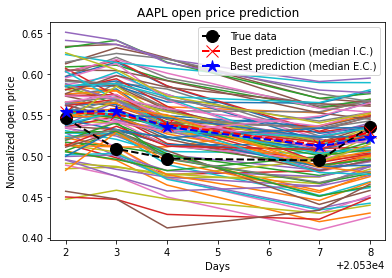
\includegraphics[height=0.45\textheight]{open_AAPL.png}
	Prediction of AAPL open price.
	\end{column}%

	\begin{column}{.5\textwidth}
	\centering
	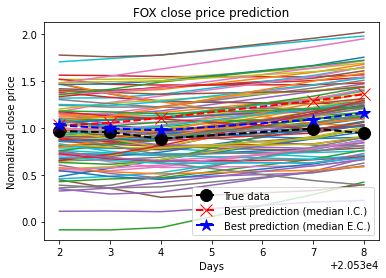
\includegraphics[height=0.45\textheight]{close_FOX.png}
	Prediction of FOX close price.
	\end{column}
	\end{columns}

	\hfill \break

	\centering
	\begin{tabular}{|c|c|c|} \hline
	& MAE on Median I.C. & MAE on Median E.C. \\
	\hline
	AAPL & 0.0051 & 0.0066 \\
	\hline
	FOX & 0.1836 & 0.3016 \\
	\hline
 	\end{tabular}

\end{frame}
%---------------------------------------------%
%% SLIDE 1.17.2:
\begin{frame}
	\frametitle{Results}
	\begin{columns}
	\begin{column}{.5\textwidth}
	\centering
	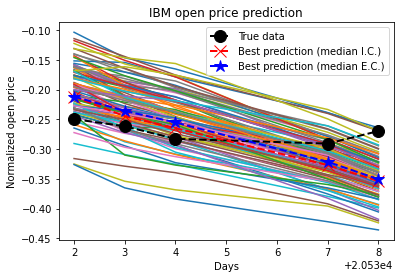
\includegraphics[height=0.45\textheight]{open_IBM.png}
	Prediction of IBM open price.
	\end{column}%

	\begin{column}{.5\textwidth}
	\centering
	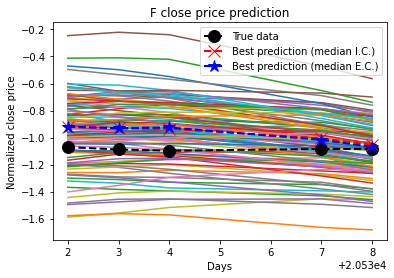
\includegraphics[height=0.45\textheight]{close_F.png}
	Prediction of F close price.
	\end{column}
	\end{columns}

	\hfill \break

	\centering
	\begin{tabular}{|c|c|c|} \hline
	& MAE on Median I.C. & MAE on Median E.C. \\
	\hline
	IBM & 0.0086 & 0.0068 \\
	\hline
	F & 0.0311 & 0.0347 \\
	\hline
 	\end{tabular}

\end{frame}
%---------------------------------------------%
%% SLIDE 1.18:
\begin{frame}
	\frametitle{Final remarks and future work (1)}
	\framesubtitle{Just one -- even successful -- try is never enough!}

	\begin{displayquote}
		“We never wanted to build an infallible oracle, but just to ease risk management.”
		\begin{flushright}Ritchie Ng (Chief of AI -- Hessian Matrix Capital) \end{flushright}
	\end{displayquote}

\end{frame}


\begin{frame}
	\frametitle{Final remarks and future work (2)}
	\framesubtitle{Just one -- even successful -- try is never enough!}

	Overall, a moderately-successful application of \textit{state-of-the-art} NN methods to a real-world problem, despite the lack of settled knowledge on the matter and training instabilities.
	\hfill \break
	\begin{itemize}
		\item{Fairly \textit{close-to-reality} predictions provided a successful training;}
		\item{Usable uncertainty estimation for \textit{limit-case} scenarios;}
		\item{Fast and introspectable training ($\leftarrow$ heuristics).}
	\end{itemize}
	\hfill \break
	Not a perfect one, though...
	\hfill \break
	\begin{itemize}
		\item{Extreme brittleness of hyperparameter tuning;}
		\item{Too broad uncertainty for finer-grained analysis;}
		\item{Deep $\mathcal{L}$ local minima may require training restart.}
	\end{itemize}

\end{frame}
}

%% THANKS!
\begin{frame}
	\frametitle{Greetings}
	\center Thank you for your attention!
	%\hfill\break
%	\hfill\break
	\center 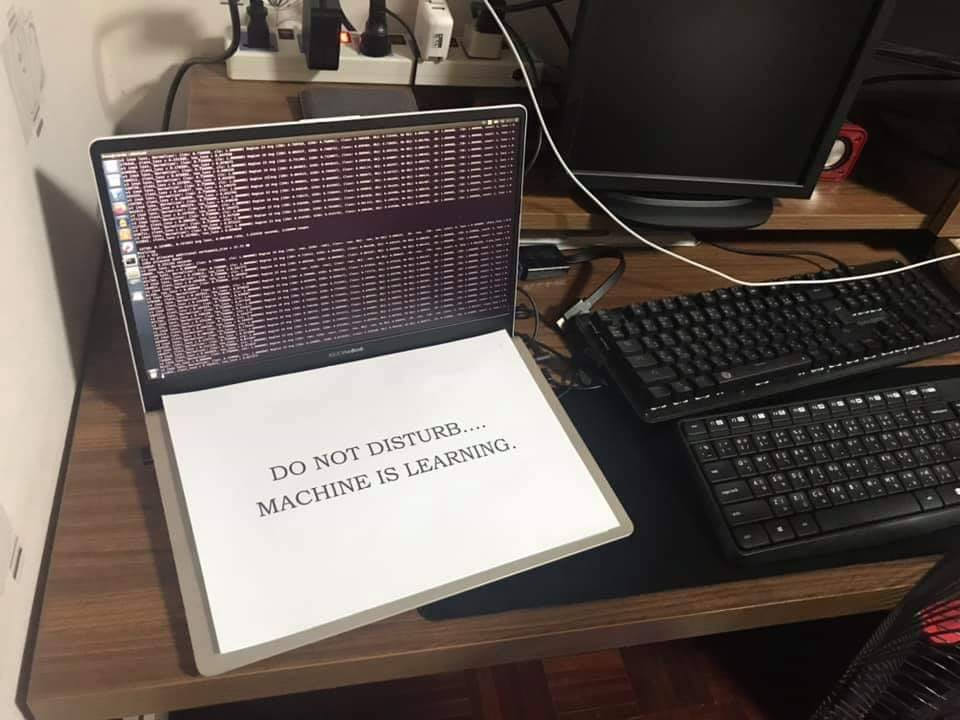
\includegraphics[scale = 0.21]{dndmil.jpeg}
	\center \url{https://github.com/emaballarin/cathode}
\end{frame}

%-----------------------------------------------%
%-----------------------------------------------%
\end{document}

